\section{Technical preliminaries}\label{sec:prelims}

\begin{figure*}
    \centering
    \begin{subfigure}[b]{0.49\textwidth}
        \centering
        \scalebox{0.7}{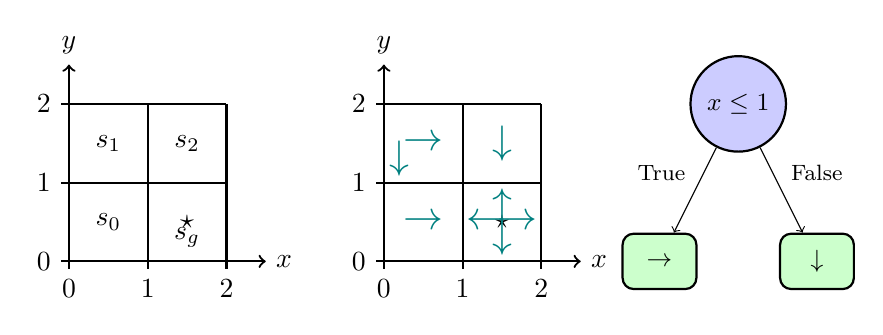
\begin{tikzpicture}[
        decision/.style={circle, draw, thick, fill=blue!20, text width=2.5em, text centered, minimum height=2.5em, font=\small},
        leaf/.style={rectangle, draw, thick, fill=green!20, text width=2em, text centered, rounded corners, minimum height=2em, font=\small},
        edge_label/.style={font=\footnotesize, midway}
    ]
        \tikzstyle{grid}=[draw, thick, fill=gray!10]
        
        % Draw grid
        \draw[grid] (0,0) grid (2,2);
        
        % Add axes
        \draw[thick, ->] (0,0) -- (2.5,0) node[right] {$x$};
        \draw[thick, ->] (0,0) -- (0,2.5) node[above] {$y$};
        
        % Add tick marks and labels
        \foreach \x in {0,1,2} {
            \draw[thick] (\x,0) -- (\x,-0.1) node[below] {$\x$};
        }
        \foreach \y in {0,1,2} {
            \draw[thick] (0,\y) -- (-0.1,\y) node[left] {$\y$};
        }
        
        % Add state labels clockwise from bottom left
        \node at (0.5,0.5) {$s_0$};
        \node at (1.5,0.5) {$\star$};
        \node at (1.5,0.3) {$s_g$};
        \node at (1.5,1.5) {$s_2$};
        \node at (0.5,1.5) {$s_1$};

        % Draid
        \draw[grid] (4,0) grid (6,2);
    
        % Adds
        \draw[thick, ->] (4,0) -- (6.5,0) node[right] {$x$};
        \draw[thick, ->] (4,0) -- (4,2.5) node[above] {$y$};
    
        % Addk marks and labels
        \draw[thick] (4,0) -- (4,-0.1) node[below] {$0$};
        \draw[thick] (5,0) -- (5,-0.1) node[below] {$1$};
        \draw[thick] (6,0) -- (6,-0.1) node[below] {$2$};
    

        \foreach \y in {0,1,2} {
            \draw[thick] (4,\y) -- (3.9,\y) node[left] {$\y$};
        }
        
        % Add state labels clockwise from bottom left
        \node at (4.5,0.5) {\Large{\color{teal} $\boldsymbol{\rightarrow}$}};
        \node at (5.5,0.5) {$\star$};
        \node at (5.5,0.7) {\Large{\color{teal} $\boldsymbol{\uparrow}$}};
        \node at (5.5,0.3) {\Large{\color{teal} $\boldsymbol{\downarrow}$}};
        \node at (5.7,0.5) {\Large{\color{teal} $\boldsymbol{\rightarrow}$}};
        \node at (5.3,0.5) {\Large{\color{teal} $\boldsymbol{\leftarrow}$}};
        \node at (5.5,1.5) {\Large{\color{teal} $\boldsymbol{\downarrow}$}};
        \node at (4.2,1.3) {\Large{\color{teal} $\boldsymbol{\downarrow}$}};
        \node at (4.5,1.5) {\Large{\color{teal} $\boldsymbol{\rightarrow}$}};
        
        \node[decision] (tree5_root) at (8.5,2) {$x \leq 1$};
        \node[leaf] (tree5_right) at (7.5,0) {$\rightarrow$};
        \node[leaf] (tree5_left) at (9.5,0) {$\downarrow$};
        \draw[->] (tree5_root) -- (tree5_right) node[edge_label, above left] {True};
        \draw[->] (tree5_root) -- (tree5_left) node[edge_label, above right] {False};
        \tikzstyle{grid}=[draw, thick, fill=gray!10]
        \end{tikzpicture}}
        \caption{{\small MDP, optimal actions, and an optimal decision tree policy}}\label{fig:mdp-dt}
    \end{subfigure}
    \hfill
    \begin{subfigure}[b]{0.49\textwidth}
        \centering
        \scalebox{0.7}{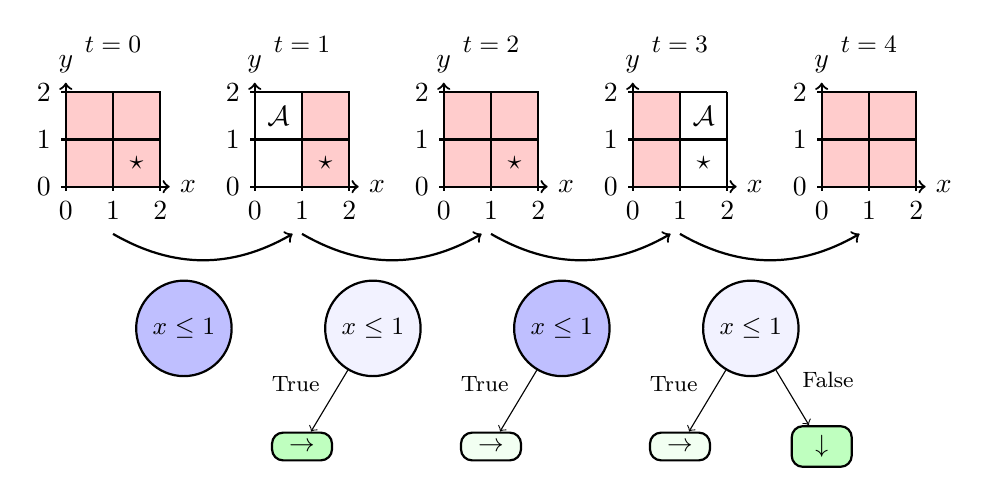
\begin{tikzpicture}[scale=0.6]
    % Define styles
    \tikzstyle{grid}=[draw, thick, fill=gray!10]
    \tikzstyle{rectangle}=[draw, thick, fill=red!20]
    
    % Row 1: IBMDP States (s, o)
    % t=0: Initial state
    \node at (2,7) {\small $t=0$};

    \draw[rectangle] (1,4) rectangle (3,6);
    \draw[grid] (1,4) grid (3,6);
    % Add axes
    \draw[thick, ->] (1,4) -- (3.2,4) node[right] {$x$};
    \draw[thick, ->] (1,4) -- (1,6.2) node[above] {$y$};
    \foreach \x in {0,1,2} {
        \draw[thick] (\x+1,4) -- (\x+1,3.9) node[below] {$\x$};
    }
    \foreach \y in {0,1,2} {
        \draw[thick] (1,\y+4) -- (0.9,\y+4) node[left] {$\y$};
    }
    \node at (2.5, 4.5) {$\star$};
    % \node at (1.5, 5.5) {$\mathcal{A}$};
    
    % Curved arrow from t=0 to t=1
    \draw[thick, ->] (2,3) to[bend right=30] node[midway, below] {} (5.8,3);

    % % t=1: After AIG x≤0.5
    \node at (6,7) {\small $t=1$};

    \draw[rectangle] (6,4) rectangle (7,6);
    \draw[grid] (5,4) grid (7,6);
    % Add axes
    \draw[thick, ->] (5,4) -- (7.2,4) node[right] {$x$};
    \draw[thick, ->] (5,4) -- (5,6.2) node[above] {$y$};
    \foreach \x in {0,1,2} {
        \draw[thick] (\x+5,4) -- (\x+5,3.9) node[below] {$\x$};
    }
    \foreach \y in {0,1,2} {
        \draw[thick] (5,\y+4) -- (4.9,\y+4) node[left] {$\y$};
    }
    \node at (6.5, 4.5) {$\star$};
    \node at (5.5, 5.5) {$\mathcal{A}$};



    % Curved arrow from t=1 to t=2
    \draw[thick, ->] (6,3) to[bend right=30] node[midway, below] {}(9.8,3);

    \node at (10,7) {\small $t=2$};
    
    \draw[rectangle] (9,4) rectangle (11,6);
    \draw[grid] (9,4) grid (11,6);
    % Add axes
    \draw[thick, ->] (9,4) -- (11.2,4) node[right] {$x$};
    \draw[thick, ->] (9,4) -- (9,6.2) node[above] {$y$};
    \foreach \x in {0,1,2} {
        \draw[thick] (\x+9,4) -- (\x+9,3.9) node[below] {$\x$};
    }
    \foreach \y in {0,1,2} {
        \draw[thick] (9,\y+4) -- (8.9,\y+4) node[left] {$\y$};
    }
    \node at (10.5, 4.5) {$\star$};
    % \node at (12.5, 5.5) {$\mathcal{A}$};

    
    % Curved arrow from t=2 to t=4
    \draw[thick, ->] (10,3) to[bend right=30] node[midway, below] {} (13.8,3);
    
    \node at (14,7) {\small $t=3$};

    \draw[rectangle] (13,4) rectangle (14,6);
    \draw[grid] (13,4) grid (15,6);
    % Add axes
    \draw[thick, ->] (13,4) -- (15.2,4) node[right] {$x$};
    \draw[thick, ->] (13,4) -- (13,6.2) node[above] {$y$};
    \foreach \x in {0,1,2} {
        \draw[thick] (\x+13,4) -- (\x+13,3.9) node[below] {$\x$};
    }
    \foreach \y in {0,1,2} {
        \draw[thick] (13,\y+4) -- (12.9,\y+4) node[left] {$\y$};
    }
    \node at (14.5, 4.5) {$\star$};
    \node at (14.5, 5.5) {$\mathcal{A}$};

    
    \draw[thick, ->] (14,3) to[bend right=30] node[midway, below] {} (17.8,3);
    
    % % \node[circle, draw, thick, fill=blue!25, text width=2em, text centered, minimum height=1.5em, font=\small] (tree4_root) at (14.5,0) {$x \leq 1$};
    % % \node[rectangle, draw, thick, fill=green!5, text width=1.5em, text centered, rounded corners, minimum height=1em, font=\small] (tree4_right) at (13,-3) {$\rightarrow$};
    % % \node[rectangle, draw, thick, fill=green!5, text width=1.5em, text centered, rounded corners, minimum height=1em, font=\small] (tree4_left) at (16,-3) {$\downarrow$};
    % % \draw[->] (tree4_root) -- (tree4_right) node[font=\footnotesize, midway, above left] {True};
    % % \draw[->] (tree4_root) -- (tree4_left) node[font=\footnotesize, midway, above right] {False};


    \node at (18,7) {\small $t=4$};
 
    \draw[rectangle] (17,4) rectangle (19,6);
    \draw[grid] (17,4) grid (19,6);
    % % Add axes
    \draw[thick, ->] (17,4) -- (19.2,4) node[right] {$x$};
    \draw[thick, ->] (17,4) -- (17,6.2) node[above] {$y$};
    \foreach \x in {0,1,2} {
        \draw[thick] (\x+17,4) -- (\x+17,3.9) node[below] {$\x$};
    }
    \foreach \y in {0,1,2} {
        \draw[thick] (17,\y+4) -- (16.9,\y+4) node[left] {$\y$};
    }
    % \node at (18.5, 4.5) {$\star$};
    % \node at (18.6, 4.6) {$\mathcal{A}$};


    % \node[circle, draw, thick, fill=blue!5, text width=2em, text centered, minimum height=1.5em, font=\small] (tree4_root) at (19.5,0) {$x \leq 1$};
    % \node[rectangle, draw, thick, fill=green!5, text width=1.5em, text centered, rounded corners, minimum height=1em, font=\small] (tree4_right) at (18,-3) {$\rightarrow$};
    % \node[rectangle, draw, thick, fill=green!25, text width=1.5em, text centered, rounded corners, minimum height=1em, font=\small] (tree4_left) at (21,-3) {$\downarrow$};
    % \draw[->] (tree4_root) -- (tree4_right) node[font=\footnotesize, midway, above left] {True};
    % \draw[->] (tree4_root) -- (tree4_left) node[font=\footnotesize, midway, above right] {False};
    \node[circle, draw, thick, fill=blue!5, text width=2.5em, text centered, minimum height=2.5em, font=\small] (tree4_root) at (15.5,1) {$x \leq 1$};
    \node[rectangle, draw, thick, fill=green!5, text width=1.5em, text centered, rounded corners, minimum height=1em, font=\small] (tree4_right) at (14,-1.5) {$\rightarrow$};
    \node[rectangle, draw, thick, fill=green!25, text width=1.5em, text centered, rounded corners, minimum height=1em, font=\small] (tree4_left) at (17,-1.5) {$\downarrow$};
    \draw[->] (tree4_root) -- (tree4_right) node[font=\footnotesize, midway, above left] {True};
    \draw[->] (tree4_root) -- (tree4_left) node[font=\footnotesize, midway, above right] {False};

    % \node[circle, draw, thick, fill=blue!25, text width=2em, text centered, minimum height=1.5em, font=\small] (tree4_root) at (26.5,5) {$x \leq 1$};
    % \node[rectangle, draw, thick, fill=green!25, text width=1.5em, text centered, rounded corners, minimum height=1em, font=\small] (tree4_right) at (25,2) {$\rightarrow$};
    % \node[rectangle, draw, thick, fill=green!25, text width=1.5em, text centered, rounded corners, minimum height=1em, font=\small] (tree4_left) at (28,2) {$\downarrow$};
    % \draw[->] (tree4_root) -- (tree4_right) node[font=\footnotesize, midway, above left] {True};
    % \draw[->] (tree4_root) -- (tree4_left) node[font=\footnotesize, midway, above right] {False};


    \node[circle, draw, thick, fill=blue!25, text width=2.5em, text centered, minimum height=2.5em, font=\small] (tree4_root) at (11.5,1) {$x \leq 1$};
    \node[rectangle, draw, thick, fill=green!5, text width=1.5em, text centered, rounded corners, minimum height=1em, font=\small] (tree4_right) at (10,-1.5) {$\rightarrow$};
    % \node<6->[rectangle, draw, thick, fill=green!5, text width=1.5em, text centered, rounded corners, minimum height=1em, font=\small] (tree4_left) at (16,-3) {$\downarrow$};
    \draw[->] (tree4_root) -- (tree4_right) node[font=\footnotesize, midway, above left] {True};
    % \draw<6->[->] (tree4_root) -- (tree4_left) node[font=\footnotesize, midway, above right] {False};

    \node[circle, draw, thick, fill=blue!5, text width=2.5em, text centered, minimum height=2.5em, font=\small] (tree4_root) at (7.5,1) {$x \leq 1$};
    \node[rectangle, draw, thick, fill=green!25, text width=1.5em, text centered, rounded corners, minimum height=1em, font=\small] (tree4_right) at (6,-1.5) {$\rightarrow$};
    \draw[->] (tree4_root) -- (tree4_right) node[font=\footnotesize, midway, above left] {True};

    \node[circle, draw, thick, fill=blue!25, text width=2.5em, text centered, minimum height=2.5em, font=\small] (tree4_root) at (3.5,1) {$x \leq 1$};
    % \node<5>[rectangle, draw, thick, fill=green!5, text width=1.5em, text centered, rounded corners, minimum height=1em, font=\small] (tree4_right) at (3,-3) {$\rightarrow$};
    % \node<5>[rectangle, draw, thick, fill=green!5, text width=1.5em, text centered, rounded corners, minimum height=1em, font=\small] (tree4_left) at (6,-3) {$\downarrow$};
    % \draw<5>[->] (tree4_root) -- (tree4_right) node[font=\footnotesize, midway, above left] {True};
    % \draw<5>[->] (tree4_root) -- (tree4_left) node[font=\footnotesize, midway, above right] {False};

    
\end{tikzpicture}}
        \caption{{\small An associated IBMDP trajectory.}}\label{fig:ibmdp-example}
    \end{subfigure}
    \caption{Figure~\ref{fig:mdp-dt} shows a four-state grid world MDP with four directional actions and zero reward except at the goal state ($\star$). The center illustrates an optimal policy, and the right an optimal depth-1 decision tree that tests state coordinates to choose actions. Figure~\ref{fig:ibmdp-example} depicts an IBMDP trajectory for this grid world. Observations $\boldsymbol{o}_t$ encode bounds on the agent’s unknown state features: initially $\boldsymbol{o}_0=(0,2,0,2)$ (“the state could be anywhere”). Information-gathering actions iteratively refine these bounds, corresponding to internal tree tests. For example, at $t=0$ the IGA $\langle x,1\rangle$ yields reward $\zeta$ and updates the observation to $\boldsymbol{o}_1=(0,1,0,2)$. A downstream action then moves the agent, gives reward 0, resets the bounds, and the process repeats until reaching the absorbing goal state. Masking the true state forces the agent to gather information to act optimally.}
\end{figure*}

\subsection{Markov decision processes}

Markov decision processes were first introduced in the 1950s by Richard Bellman~\cite{Bellman}.
Informally, an MDP models how an agent acts over time to achieve a goal. 
At every time step, the agent observes its current state (e.g., patient weight and tumor size) and takes an action (e.g., administers a certain amount of chemotherapy).
The agent receives a reward that helps evaluate the quality of the action with respect to the goal (e.g., tumor size decrease when the objective is to cure cancer).
Finally, the agent transitions to a new state (e.g., the updated patient state) and repeats this process over time:
\begin{definition}[Markov decision process]\label{def:mdp} An MDP is a tuple $\mathcal{M} = \langle S, A, R, T, T_0 \rangle$.
$S$ is a finite set of states representing all possible configurations of the environment.
$A$ is a finite set of actions available to the agent.
$R: S \times A \rightarrow \mathbb{R}$ is a deterministic reward function that assigns a real-valued reward to each state-action pair. While in general reward functions are often stochastic, in this manuscript we focus deterministic ones without loss of generality.
$T: S \times A \rightarrow \Delta(S)$ is the transition function that maps state-action pairs to probability distributions over next states $\Delta(S)$.
$T_0 \in \Delta(S)$ is the initial distribution over states.
\end{definition}

Informally, we would like to act in an MDP so that we obtain as much reward as possible over time.
We can formally define this objective, that we call the reinforcement learning objective, as follows:

\begin{definition}[Reinforcement learning objective]\label{def:mdp-obj} Given an MDP (definition~\ref{def:mdp}) $\mathcal{M}\equiv\langle S, A, R, T, T_0 \rangle$, the goal of reinforcement learning for sequential decision making is to find a model, also known as a policy, $\pi: S \rightarrow A$ that maximizes the expected discounted sum of rewards:
{\small
$$J(\pi) = \mathbb{E}\left[\sum_{t=0}^{\infty} \gamma^t R(s_t, \pi(s_t)) \mid s_0 \sim T_0, s_{t+1} \sim T(s_t, \pi(s_t))\right]$$}
where $0< \gamma\leq 1$ is the discount factor that controls the trade-off between immediate and future rewards.
\end{definition}

Algorithms presented in this article aim to find an optimal policy $\pi^\star \in\underset{\pi}{\operatorname{argmax}}\ J(\pi)$ that maximizes the above reinforcement learning objective.
In particular, RL algorithms~\cite{sutton,pg_sutton,watkins1992q,dqn,ppo} learn such optimal policies using data of MDP interactions without prior knowledge of the reward and transition models.
Useful quantities for such algorithms include \textit{value} of states and actions.
\begin{definition}[Value of a state]\label{def:vs} 
    In an MDP $\mathcal{M}$ (definition~\ref{def:mdp}), the value of a state $s\in S$ under policy $\pi$ is the expected discounted sum of rewards starting from state $s$ and following policy $\pi$:
    {\small
    $$V^\pi(s) = \mathbb{E}\left[\sum_{t=0}^{\infty} \gamma^t R(s_t, \pi(s_t)) \mid s_0 = s, s_{t+1} \sim T(s_t, \pi(s_t))\right]$$}
    Applying the Markov property gives a recursive definition of the value of $s$ under policy $\pi$: $V^\pi(s) = R(s,\pi(s)) + \gamma \mathbb{E}\left[V^\pi(s') | s'\sim T(s, \pi(s))\right]$.
    The optimal value of a state $s\in S$, $V^\star(s)$, is the value of state $s$ when following the optimal policy $\pi^{\star}$ (the policy that maximizes the RL objective (definition~\ref{def:mdp-obj})): $V^{\star}(s) = V^{\pi^{\star}}(s)$.
    Similarly, the optimal value of a state–action pair $(s,a)\in S\times A$, $Q^\star(s,a)$, is the value when taking action $a$ in state $s$ and then following the optimal policy: $Q^{\star}(s,a) = R(s, a) + \gamma\mathbb{E}\left[V^{\star}(s') | s'\sim T(s, a)\right]$.
\end{definition}

\subsection{Decision tree policies}
While other interpretable policy classes exist~\cite{kohler2025evaluating}, one conjecture from~\citet{glanois-survey} is that interpretable models are all hard to optimize or learn because they are non-differentiable in nature.
This is something that will be key in our study of decision tree policy that we introduce next.

\begin{definition}[Decision tree policy]\label{def:dt}
    A decision tree policy is a rooted tree $\pi_{\mathcal{T}} = (\mathcal{N}, E)$.
    Each internal node $\nu \in \mathcal{N}$ is associated with a test that maps an MDP state attribute to a Boolean, e.g. $s_{i}\leq v$ for $v\in \mathbb{R}$.
    Each edge $e \in E$ from an internal node corresponds to an outcome of the associated test function.
    Each leaf node $l \in \mathcal{N}$ is associated with an MDP action $a_l \in A$.
    For any input $s \in S$, the tree defines a unique path from root to leaf, determining the prediction $\pi_{\mathcal{T}}(s) = a_l$ where $l$ is the reached leaf.
    The depth of a tree is the maximum path length from root to any leaf.
\end{definition}

In figure~\ref{fig:mdp-dt}, we present an example Markov decision process (definition~\ref{def:mdp}), the optimal actions that maximize the RL objective (definition~\ref{def:mdp-obj}), and a decision tree policy (definition~\ref{def:dt}) that also maximizes the RL objective.
Next, we present the class of MDPs introduced in~\citet{topin2021iterative} useful for our to understand reinforcement learning of decision tree policies that directly optimize the RL objective in an MDP.

\subsection{Iterative bounding Markov decision processes}\label{sec:ibmdp}
Iterative bounding MDPs (IBMDPs) are, as the name suggests, standard MDPs (definition~\ref{def:mdp}) and therefore admit optimal deterministic Markovian policies~\cite{Bellman}. We assume continuous state spaces with finite action sets, using bold notation for vector-valued states and observations (though our results also extend to discrete states).

Given a downstream MDP where we seek a decision tree policy, an IBMDP augments the state with additional observations that iteratively refine knowledge about the downstream state features. Actions include (i) downstream actions that affect the environment and receive the same rewards as in the original MDP, and (ii) information-gathering actions (IGAs) that update the observations. IGAs receive a chosen reward so that optimizing the IBMDP objective captures a trade-off between downstream performance and interpretability.

We now formally define IBMDPs following~\citet{topin2021iterative}.
\begin{definition}[Iterative bounding Markov decision process (\citet{topin2021iterative}, section 4.1)]\label{def:ibmdp}
Given a downstream MDP $\mathcal{M}\equiv\langle S, A, R, T, T_0 \rangle$ (definition~\ref{def:mdp}), an associated iterative bounding Markov decision process $\mathcal{M}_{IB}$ is a tuple:
\begin{align*}
    \langle \overbrace{S \times O}^{\text{State space}}, \overbrace{A \cup A_{info}}^{\text{Action space}}, \overbrace{(R, \zeta)}^{\text{Reward}}, \overbrace{(T_{info}, T, T_0)}^{\text{Transitions}}\rangle
\end{align*}
$S$ are the downstream MDP state features. Downstream state features $\boldsymbol{s} = (s_1, \dots, s_p)\in S$ are bounded: $s_j \in [L_j, U_j]$ where $\infty < L_j \leq U_j < \infty \ \forall 1\leq j \leq p$.
$O$ are observations. They represent bounds on the downstream state features: $O\subsetneq S^2 =  [L_1, U_1]\times \dots \times [L_p, U_p] \times [L_1, U_1]\times \dots \times [L_p, U_p]$. So the complete IBMDP state space is $S \times O$: the concatenations of downstream state features and observations.
Given some downstream state features $\boldsymbol{s} = (s_1, \dots, s_p)\in S$ and some observation $\boldsymbol{o} = (L_1, U_1, \dots, L_p, U_p)$, an IBMDP state is $\boldsymbol{s}_{IB} = (\overbrace{s_1, \dots, s_p}^{\text{downstream state features}}, \overbrace{L_1, U_1, \dots, L_p, U_p}^{\text{observation}})$.
$A$ are the downstream MDP actions.
$A_{info}$ are \textit{information-gathering} actions of the form $\langle j, v \rangle$ where $j$ is a state feature index $1 \leq j \leq p$ and $v$ is a real number between $L_j$ and $U_j$. So the complete action space of an IBMDP is the set of downstream MDP actions and information-gathering actions $A \cup A_{info}$.
$R: S\times A \rightarrow \mathbb{R}$ is the downstream MDP reward function.
$\zeta$ is a reward signal for taking an information-gathering action.
So the IBMDP reward function is to get a reward from the downstream MDP if the action is a downstream MDP action or to get $\zeta$ if the action is an IGA action.
$T_{info}: S\times O \times( A_{info} \cup A )\rightarrow \Delta (S\times O)$ is the transition function of IBMDPs: 
given some observation $\boldsymbol{o}_t = (L'_1, U'_1, \dots, L'_p, U'_p) \in O$ and downstream state features $\boldsymbol{s}_t=(s'_1, s'_2, \dots, s'_p)$ if an IGA $\langle j, v \rangle$ is taken, the new observation $\boldsymbol{o}_{t+1}$ is $(L'_1, U'_1, \dots , L'_j, \min\{v, U'_j\}, \dots , L'_p, U'_p) \text{ if } s_j \leq v$ or $(L'_1, U'_1, \dots , \max\{v, L'_j\}, U'_j, \dots , L'_p, U'_p) \text{ if } s_j > v$.
If a downstream action is taken, the observation is reset to the default downstream state feature bounds $(L_1, U_1,\dots, L_p, U_p)$ and the downstream state features change according to the downstream MDP transition function: $\boldsymbol{s}_{t+1}\sim T(\boldsymbol{s}_t, a_t)$.
At initialization, the downstream state features are drawn from the downstream MDP initial distribution $T_0$ and the observation is always set to the default downstream state features bounds $\boldsymbol{o}_0=(L_1, U_1,\dots, L_p, U_p)$.
\end{definition}

We present an IBMDP for a the grid-world MDP (figure~\ref{fig:mdp-dt}) in figure~\ref{fig:ibmdp-example}.
Now remains to extract a decision tree policy (definition~\ref{def:dt}) for a downstream MDP $\mathcal{M}$ from a policy for an associated IBMDP $\mathcal{M}_{IB}$. 

\subsection{From policies to trees}
information-gathering actions (definition~\ref{def:ibmdp}) resemble the tests $1_{\{x_{\_, j} \leq v\}}$ that make up internal decision tree nodes (figure~\ref{fig:ibmdp-example}).
Indeed, a policy taking actions in an IBMDP essentially builds a tree by taking sequences of IGAs (internal nodes) and then a downstream action (leaf node) and repeats this process over time.
In particular, the IGA rewards $\zeta$ can be seen as a regularization or a penalty for interpretability: if $\zeta$ is very small compared to downstream rewards, a policy will try to take downstream actions as often as possible, i.e. build shallow trees with short paths between root and leaves.

\citet{topin2021iterative} show that only a subset of IBMDP policies correspond to downstream decision tree policies. Their extraction algorithm (algorithm~\ref{alg:extract-tree}) requires deterministic policies that depend only on IBMDP observations. Non-deterministic policies would yield stochastic decision trees~\cite{stoch-decision}, whose interpretability remains unclear. Policies that depend on the full IBMDP state also defeat the purpose of information-gathering actions, since the agent already has all necessary state information to act optimally.
The connections between partially observable MDPs (POMDPs~\cite{POMDP,chap2}) and extracting decision tree policies from IBMDPs might seem obvious but they are absent from the original IBMDP paper~\cite{topin2021iterative} and from subsequent work.
In the next section we bridge this gap.